\chapter{Conclusion and Interesting Directions}
\label{chap:future}

In this dissertation, we investigated the use of neural networks as digital representations of media objects in multiple resolutions. Neural networks offer a model to approximate continuous functions, bridging the gap between the mathematical universe of modeling and the implementation universe, in the paradigm of the four universes. The current scenario where specific hardware as neural engines are being designed and comercilaized for consumer products as laptops, smartphones, smartwatches, VR headsets or even AR glasses, we believe that neural assets will play an important role in multiple industries.  In particular, we envision a future where neural networks will be standard digital representations of assets for particular applications in the audiovisual or games indutries.


constituting what we call representational networks.

In this dissertation we have contributed to the understanding of the frequencies in sinusoidal neural networks and their connection to the multiresolution analysis theory. We have presented MR-Net as a family of architectures to encode signals in multiresolution showcansing its applications in media objects such as images and material textures. MR-Net is available as a software component, a flexible framework that implements the architectures described in Chapter \ref{chap:mr_snn} and the multiresolution training of the networks. It can be found in \ref{}. Additionaly We demonstrated how to create periodic sinusoidal neural networks to represent periodic textures, we develop a techinique based on Poisson Equation to create seamless material textures, and we demonstrated how to use our architecture for rendering of textured objects.

Next, we explore some limitations and interesting research directions related to our work.

\section{Limitations}

\subsection{Frequencies}

By understanding the relationship between initialiation of the first sinusoidal layer of a sinusoidal neural network and the frequencies learned by the model, we have made significant progress into connecting an emprirical hyperparameter to the Shannon-Nyquist theory. Moreover, we concluded that using interger frequencies is more appropriate as it has an underlying model that constitutes a representation for a well defined function space (periodic functions) and we can reduce the space of possible values for the initialiation to a discrete a finite set o values, thus helping on the design of a initialization strategy. 

However, there are two limitations that we believe should be addressed in future works. First, is that the frequencies of the first layer of the network need to be kep frozen during the training, working similarly to a Fourier Feature Mapping with only sines. Deriving a way of making these frequencies learnable while guarateeing that these values are kep as integers is a desirable progress. This could lead to better performing models.

Second, the frequencies are still chosen in a random way with an empirical choice based on the a fraction of the Nyquist limit. Works like \cite{tamingFactory} may help to solve this problem by exploring the harmonic expansion of the frequencies generated in a sinusoidal network and providing ways of bounding these frequencies.

\subsection{Implicit Representations}

Related to the frequencies choice, we would like to discuss the implicit represnetations of media, that is representing an object as a level set of an implicit function. We presented experiemnts for one-dimensional signals, that could be related to audio waves, and image signals. We have also experimented with higher order signals as it will be discussed in REFFFFFFFFF. However, all these media objects are represented explicitly as scalar or vector fields. In these cases, we can sample the signal uniformly and we have the support of the Shannon-Nyquist theory to guide our choices of initiaization of the networks.

For objects defined implicitly such as shapes given by a signed distance function or unsigned distance function, the relationship between the samples and the frequencies or even methods for filtering and building a multiscale representation are not straighforward. Works like MIP-PLICITS show that it is possible to and fruitful to decompose these signals and use a multistage network to represent them, but the terrain for choosing hyperparameters may be more unccertain.

\subsection{Compression}

Thinking of a useful digital represnetation we must make sure it is compact and lightweight to store in the disk or transmiti through the network. Part of this is due to small neural networks architectures, that is, managing to encode signals using networks with less weights. This part was a concern in this dissertation. However, this alone is not sufficient as the size of an image file is not only determided by the amaount of values it has to store, being either the total of pixels in a matrix or the total of weights in a network, but also by the level of compression.

In this sense, it is important to couple these results to efficient compression methods for neural networks such as COIN, COIN++ or even develop new methods for this goal.


\section{Interesting Directions}


\subsection{Volumetric Textures}


Show experiments

\subsection{Hypertextures}

Perlin...

\subsection{Irregular sampling}

Poisson disc sampling

Panorama

\subsection{Transformations}

Morphing, Video...


\section{Closure}

dsdsdsdsddsd



% % \subsubsection{Sampling}
% % The input for the neural network is a discrete representation. In this sense,} sampling is a way to create a representation of a function based on its values at certain points of the domain. From the point of view of Representation Theory, we can interpret this as a projection of the function onto the primal Shannon basis (i.e., Dirac delta distribution). In the context of signal processing, this basis is a sampling grid of impulses and the representation consists of the sequence of signal values at the grid locations.

% % One important aspect of sampling for learning signals with coordinate-based neural network is the structure of the sampling grid. In that respect, it is instrumental to consider two types of grid structures: Regular and Irregular. See Fig~\ref{f:sampling}. {\color{red}The sampling mode is stored in the MR-Structure, so it can be taken into account when doing operations that modify the sampling grid.}

% % \begin{figure}[!h]
% % \centering
% % 
\includegraphics[width=0.42\linewidth]{img/ch4/regular.png}
% % \hfil
% % 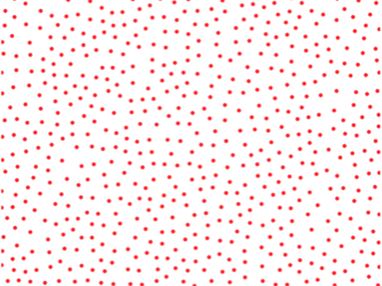
\includegraphics[width=0.42\linewidth]{img/ch4/poisson.png}
% % \\
% % {\hfil (regular grid) \hfil\hfil (irregular grid) \hfil}
% % \caption{Sampling Modes}
% % \label{f:sampling}
% % \end{figure}


% % \subsubsection{Filtering}

% % The input of signal values to the network can be filtered to separate it into different frequency bands. In this sense, we can use the unfiltered signal, a low-pass version of the signal or a band-pass version of the signal. See Fig~\ref{f:filter}.

% % It is common to employ a Gaussian Kernel as the low-pass Kernel and a Difference of Gaussians as the band-pass kernel.

% % \begin{figure}[!h]
% % \centering
% % 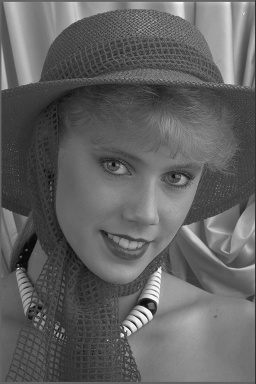
\includegraphics[width=0.30\linewidth]{img/ch4/signal.png}
% % 
\includegraphics[width=0.30\linewidth]{img/ch4/gaussian.png}
% % 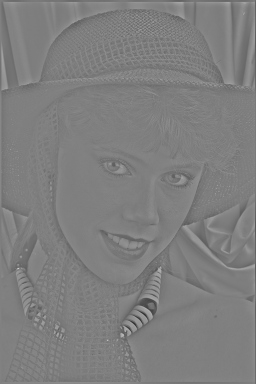
\includegraphics[width=0.30\linewidth]{img/ch4/laplacian.png}\\
% % {\hfil \hfil signal \hfil \hfil \hfil low-pass \hfil \hfil \hfil band-pass \hfil}
% % \caption{Filter Types}
% % \label{f:filter}
% % \end{figure}

% % \subsubsection{multi-stage stack}

% % A Multiresolution Stack consists of a hierarchy of sampling grids with different resolutions. The standard grid structure form a dyadic lattice of regular grids obeying the $2^j$ rule, i.e., each level of the grid has twice the size of the previous one. 
% % Nonetheless, it is also possible to define a irregular multiresolution grid structure. In this case, each resolution level has approximately twice the number of random sample points of the previous level (see Fig~\ref{f:multi}(b)).
% % On the other hand, it is possible to have a stack of sampling grid with the same resolution, in which the signal is the same at each level or is filtered (see Fig~\ref{f:multi}(a)). Section~\ref{s:lod} gives more details on this option.
% % \begin{figure}[!h]
% % \centering
% % 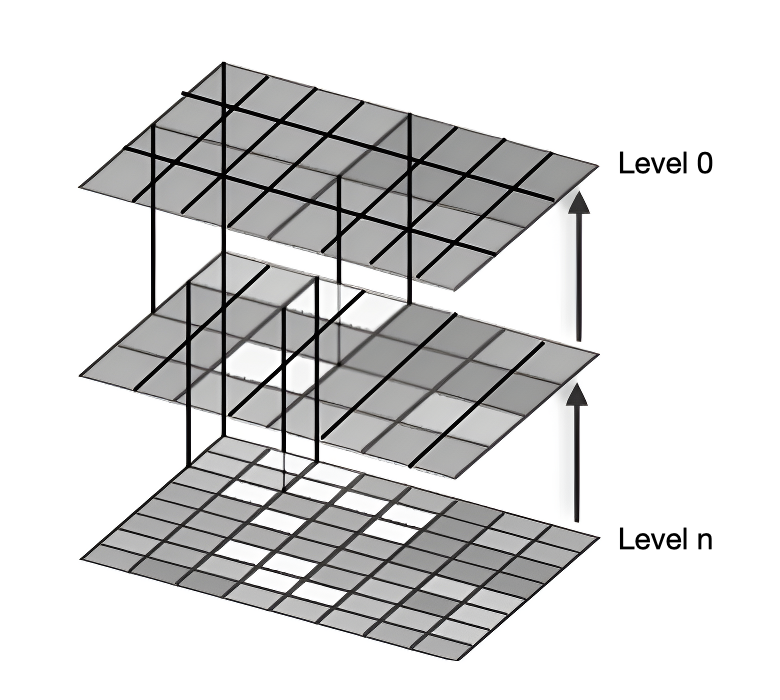
\includegraphics[width=0.45\linewidth]{img/ch4/tower.png}
% % 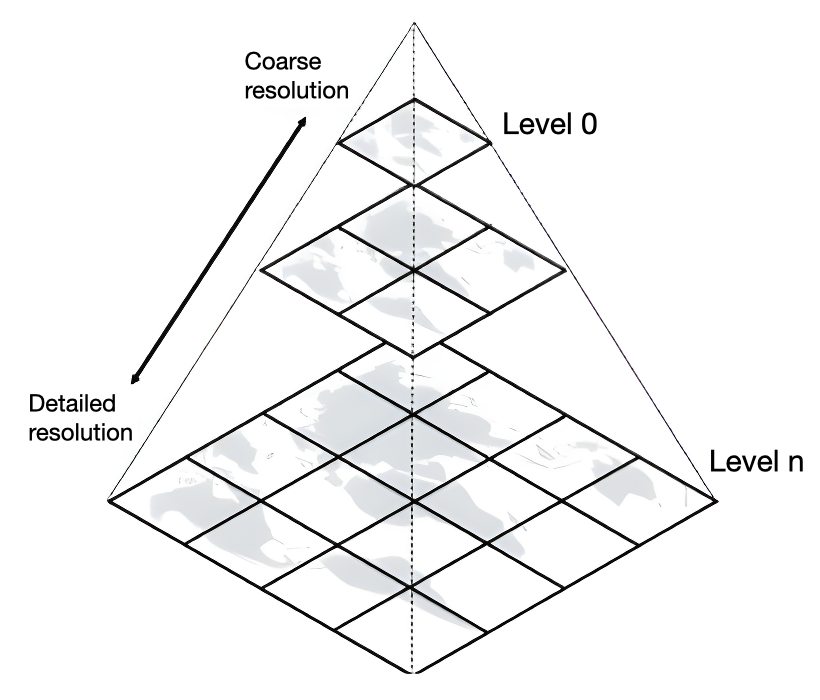
\includegraphics[width=0.45\linewidth]{img/ch4/pyramid.png}\\
% % {\hfil tower \hfil \hfil \hfil pyramid \hfil}
% % \vspace{-0.2cm}
% % \caption{\hl{Multiresolution Hierarchies}}
% % \label{f:multi}
% % \end{figure}


% % \subsection{Solid Texture Mapping}

% % Solid textures offer practical advantages as they eliminate the need for computing $uv$-coordinates on a surface. We trained a solid texture of a marble using Perlin Noise as described in section \ref{s-multires-3d}, and we integrated our representation into the Omniverse platform, which provides a comprehensive rendering pipeline management system. Figure \ref{f:solid_texture_mapping} showcases some of the results achieved using our solid texture mapping approach.

% % \begin{figure}[!h]
% % \centering
% % 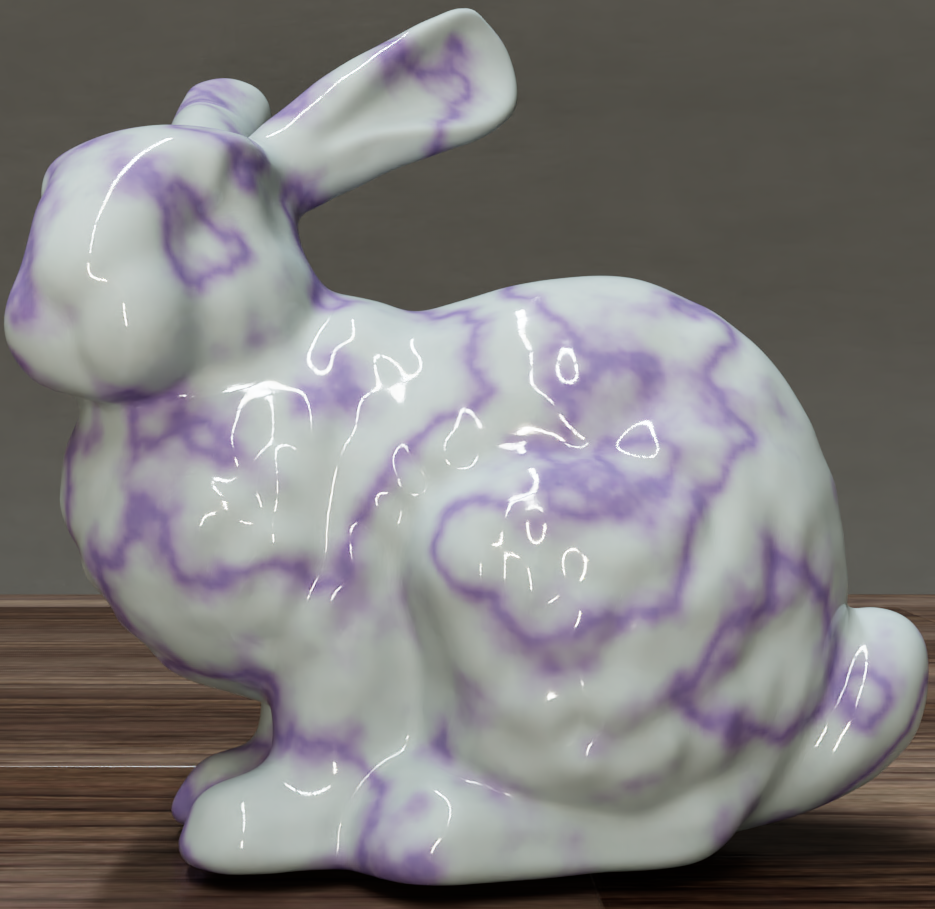
\includegraphics[width=0.375\linewidth]{img/omniverse/bunny_mrnet.0000.png}
% % 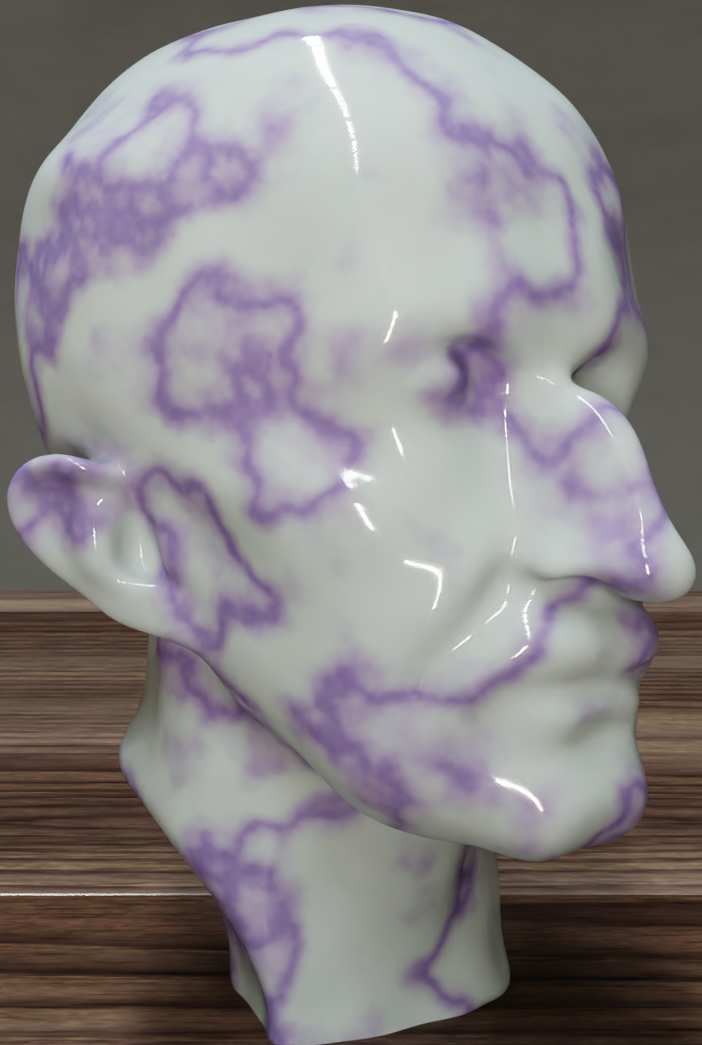
\includegraphics[width=0.245\linewidth]{img/omniverse/max_plank_mrnet_512_mc400.0099.png}
% % 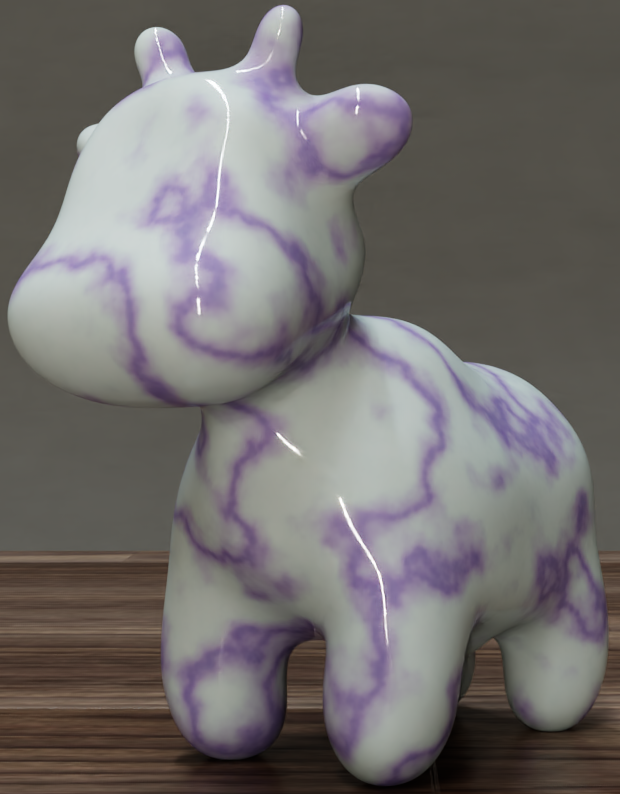
\includegraphics[width=0.285\linewidth]{img/omniverse/spot_mrnet.0101.png}
% % \caption{Solid Texture Mapping.}
% % \label{f:solid_texture_mapping}
% % \end{figure}

% % To apply the solid texture, we extract meshes from implicit surfaces represented by neural networks and perform the inference of the texture network at the vertices of the mesh. We render the scene using \textit{path tracing}, and we can choose among various materials and shading options to enhance the visual quality of the scene. This demonstrates that this approach can be fully integrated in the  graphics pipeline.

% % \end{comment}


\chapter{Conclusion}

% We have described a flexible method of working with signals in multiresolution in terms of multiple ways of preparing the input data, defining the MR-Net subclasses, and training multi-stage networks. In the applications presented in Sec. \ref{s:img}, we have explored a subset of this framework, showing cases where it improves upon existing state of the art techniques. Regarding other aspects of this groundwork, we have ongoing research on signal reconstruction from stochastic sampling, and training of L-Net models using the Laplacian pyramid, which may lead to novel imaging applications.  Some of the motivation and experiments with 1D signals in these directions are documented in \citet{supplemental}.


% In terms of future work, we plan to expand this research in two main directions. On one hand, we would like to explore the MR-Net architecture for other image applications including super-resolution, operations in the gradient domain, generation of periodic and quasi-periodic patterns, as well as image compression.
% On the other hand, we would like to extend the MR-Net representation to other media signals in higher dimensions, such as video, volumes, and implicit surfaces.

\paragraph{ORIGINAL}
Traditionally, texture tiles are depicted as discrete digital images. We propose to use our multiresolution INR to represent seamless periodic textures in a continuous, compact and fast to evaluate digital representation. In this chapter we extend deep sinusoidal neural networks to \textit{periodic neural networks} for this purpose. Inspired by the Fourier series, we constrain the representational space of our network to the space of periodic functions.

\paragraph{SUGGESTION}
In traditional approaches, textures are typically represented as discrete digital tiles, often accompanied by methods to mitigate visible seams or discontinuities when textures repeat. In contrast, this work proposes a novel approach based on implicit neural representations (INRs) to encode seamless periodic textures in a continuous and compact format that is fast to evaluate. Specifically, we extend deep sinusoidal neural networks to define \textit{periodic neural networks}, inspired by the Fourier series, which operate within the space of periodic functions.

\paragraph{FINAL VERSION}
In traditional approaches, textures are typically represented as discrete digital tiles, often accompanied by methods to mitigate visible seams or discontinuities when textures repeat. In contrast, we propose to use our multiresolution neural representation to encode seamless periodic textures in a continuous, compact and fast to evaluate digital representation. Specifically, we extend deep sinusoidal neural networks to define \textit{periodic neural networks}. Inspired by the Fourier series, we constrain the representational space of our network to the space of periodic functions.



Writing a strong conclusion chapter for your PhD dissertation is crucial to leaving a lasting impression on your readers and tying together your research. Here’s a structured approach to help you craft an effective conclusion:

1. **Restate the Research Problem and Objectives**
   - Start by summarizing the main research question or problem you tackled.
   - Reiterate the objectives you aimed to achieve, briefly reminding the reader of the purpose of your research.

2. **Summarize Key Findings**
   - Highlight the most important findings from each chapter of your dissertation. Since your work focuses on complex concepts like multiresolution neural networks and media object encoding, synthesize your results without diving into too much technical detail.
   - Emphasize how your work advances the field, such as your contributions to sinusoidal neural networks, multi-resolution representation, or periodic signal representation.

3. **Discuss Contributions and Impact**
   - Discuss the significance of your contributions, such as the development of MR-Net and other architectures like S-Net, L-Net, and M-Net.
   - Highlight any theoretical or practical advances in computer vision, computer graphics, and machine learning that emerged from your work. Explain how your multiresolution framework and hierarchical approaches offer new perspectives or solutions.

4. **Reflect on Limitations**
   - Acknowledge any limitations in your research. For example, mention aspects of your neural networks that could be improved, or how certain models like MR-Net might have scope for more efficient training strategies.
   - This shows academic honesty and sets the stage for future research.

5. **Suggest Future Research Directions**
   - Build on the limitations by suggesting areas for future exploration. Highlight open questions or challenges that still need addressing, such as enhancing model scalability or exploring new applications of your multiresolution framework.
   - Indicate potential improvements in both the theoretical and practical aspects of your contributions.

6. **Link Back to the Broader Field**
   - Contextualize your work within the broader field of AI, signal processing, and neural media representation. Discuss how your research fits into larger trends in computer vision and machine learning and how it might inspire future innovations.

7. **End with a Strong, Thoughtful Statement**
   - Conclude with a reflection on the journey of your research. Express how your findings contribute to pushing the boundaries of the field and the potential for your work to inspire future advancements.

Example Structure for Your Dissertation
Given your research in multiresolution neural networks, you might structure your conclusion like this:
1. **Introduction:** Restate the core problem of representing signals in media and the specific challenges you aimed to solve.
2. **Key Findings:** Summarize the insights gained from your models (e.g., MR-Net, S-Net) and how these contribute to signal decomposition and multiresolution learning.
3. **Impact on the Field:** Emphasize how your work bridges gaps between computer vision, computer graphics, and neural signal representation.
4. **Limitations and Future Work:** Discuss potential areas of improvement, such as further exploring implicit surfaces or improving periodic signal encoding.
5. **Broader Implications:** Reflect on how your dissertation advances foundational topics in AI and machine learning.
6. **Final Reflection:** End on an optimistic note about the future trajectory of your research area.

Would you like to discuss how to frame specific parts of your work in the conclusion?